\documentclass[../index.tex]{subfiles}

\begin{document}

\chapter{LITERATURE REVIEW}

Literature Review will discuss several concepts and technologies which will be used in the project.
There will be discussion regarding computer security concepts according to several standards,
followed by explanation of different types of firewalls and virtualization technologies, brief
explanation of Kubernetes system, and concluded with summary of the chapter.

\section{Theoretical Basis}

\section{Computer Security}

According to Paulsen \& Byers (2019), the term computer security can be described as a collection of
actions and rules which ensure confidentiality, integrity, and availability of a certain information
system property. This includes the physical hardware, underlying software, embedded firmware, and
data that is transmitted, saved, and processed.

Derived from above definition, three key objectives are introduced which are the core of computer
security:

\subsection{Confidentiality}

The concept of Confidentiality covers the following two corresponding concepts:

\begin{description}
	\item[Data confidentiality] Assures that private or confidential information is not made
		accessible or shared to unauthorized users.
	\item[Privacy] Assures that personals manage or influence the collection and storage of
		information related to them and by whom and to whom that information may be shared.
\end{description}

\subsection{Integrity}

The concept of Integrity covers the following two corresponding concepts:

\begin{description}
	\item[Data integrity] Assures that information and programs are communicated through a particular
		and authorized method.
	\item[System integrity] Assures that a system serves its purpose in an unimpaired form, free from
		deliberate or unintended unauthorized manipulation of the system.
\end{description}

\subsection{Availability}

Assures that systems work properly and service is available authorized users.

Another definition based on NIST standard FIPS 199 specifies the core of security goals for both
information and information systems as confidentiality, integrity, and availability. FIPS 199
establishes a classification of the aforementioned goals based on the condition and the
understanding of security loss:

\begin{description}
	\item[Confidentiality] The term of confidentiality can be defined as the act of maintaining legal
		restrictions on information access and sharing. This term includes the method for defending
		privacy of an individual and private information.
	\item[Integrity] The term integrity can be defined as the act of defending toward inappropriate
		modification of information which result in information destruction, including maintaining
		information non-repudiation and authenticity.
	\item[Availability] The term availability can be defined as the act of ensuring information can be
		accessed and used in reliable and promptly method.
\end{description}

While the aforementioned definition could be considered as well established, some computer security
professionals further define additional concepts to present bigger picture. Two of the most commonly
mentioned are follows:

\begin{description}
	\item[Authenticity] The characteristic of being legitimate and being able to be trusted and
		verified. This characteristic will result in confidence in the legitimacy of transmission, a
		message, or message author. This can be defined as verifying that users are the actual self that
		they claim to be and that every message received by the system originated from a reliable
		source.
	\item[Accountability] The security objectives that create the condition for actions of an object
		to be tracked down exclusively to that object. The concept includes deterrence, nonrepudiation,
		intrusion detection and prevention, and fault isolation. In addition, the concept of
		accountability also includes post-action restoration and judicial measures. As the fact that
		fully secure system is not a realistic objective, user is required to track down a security
		infringement in a system to a responsible team. Systems are required to safeguard the records of
		their own activities to allow follow up forensic examination.
\end{description}

\section{Threats and Attacks}

RFC 4949 defines four types of threat impacts and enumerates the attack types which result in every
impact:

\subsection{Unauthorized disclosure}

A situation which an individual acquires access to certain data albeit the individual is not legitimate.

\begin{description}
	\item[Exposure] An unauthorized individual is able to directly access to critical data.
	\item[Interception] An unauthorized individual interrupts critical data transmitted between
		legitimate origins and destinations.
	\item[Inference] A condition where an unauthorized individual is able to indirectly accesses
		critical data by understanding from the attributes or results of communications.
	\item[Intrusion] A condition where an unauthorized individual gains access to critical data by
		evading or beating the security guard of a system.
\end{description}

\subsection{Deception}

A condition which can lead in an authorized individual acquiring counterfeit data and assuming it to be the actual data.

\begin{description}
	\item[Masquerade] An unauthorized individual acquires access to a system or executes a harmful
		action by disguising as an authorized individual.
	\item[Falsification] A condition where an authorized individual is deceived by counterfeit data.
	\item[Repudiation] A condition where an individual tricks another by falsely denying obligation
		for a behavior.
\end{description}

\subsection{Disruption}

A condition which interrupts or prevents the intended functionality of system services and utilities.

\begin{description}
	\item[Incapacitation] Interrupts system operation by incapacitating a component of the system.
	\item[Corruption] Adversely mutates system operation by harmfully altering system data or functions.
	\item[Obstruction] A condition where system operation is being impeded by a threat which result in
		interruption of system services.
\end{description}

\subsection{Usurpation}

A condition where an unauthorized individual takeover the control system services or functions.

\begin{description}
	\item[Misappropriation] A condition where an individual presume unauthorized control of physical
		or logical resource of a certain system.
	\item[Misuse] A condition which may lead a system component to execute a function or behavior that
		is harmful to the security of the system.
\end{description}

\subsection{Firewall}

A firewall is a network security system which placed between local network and the Internet to
create a managed link and act as an external layer of security or boundary. The purpose of this
boundary is to safeguard the internal network from varying types of network-based threat and attack.
In addition, firewall offers a centralized control point which security and monitoring are able to
be established.

\begin{figure}[h]
	\centering
	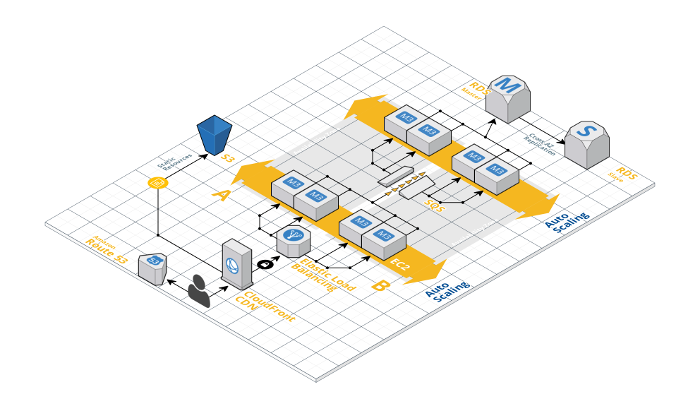
\includegraphics[width=\textwidth]{../assets/chapter-2-infrastructure-diagram.png}
	\caption{Contoh gambar}
	\label{fig:contoh_gambar}
\end{figure}

\subsection{Tabel}

Tabel juga merupakan float. Tabel~\ref{table:contoh_tabel} adalah contoh tabel. Perhatikan bahwa walaupun didefinisikan setelah paragraf ini, tabel tidak diletakkan tepat di bawah paragraf ini pada dokumen hasil kompilasi. Hal ini karena ukuran (tinggi) tabel tidak cukup apabila diletakkan di sisa halaman ini. \LaTeX-lah yang mengatur peletakan tabel. Oleh karena itu tidak disarankan untuk merujuk tabel (dan objek float lain) dengan frasa ``Tabel di bawah ini'', ``Tabel berikut'', dan sebagainya.

\begin{table}[htbp]
	\centering
	\caption{Contoh Tabel}
	\label{table:contoh_tabel}
	\begin{tabular}{ll}
		\toprule
		\multicolumn{1}{l}{\textbf{Contoh Judul Kolom}} & \multicolumn{1}{l}{\textbf{Nilai}} \\
		\midrule
		Besaran 1                                       & 12 meter                           \\
		Besaran 2                                       & $360^\circ$                        \\
		Besaran 3                                       & 0,2 meter                          \\
		Besaran 4                                       & $1^\circ$                          \\
		Besaran 5                                       & 8000 sampel/detik                  \\
		\bottomrule
	\end{tabular}
\end{table}

\section{Persamaan Matematika}

Persamaan~\eqref{eq:contoh_equation} adalah contoh persamaan matematika,

\begin{align}
	c^2 = a^2 + b^2\,.
	\label{eq:contoh_equation}
\end{align}

Contoh penggunaan notasi custom,

\begin{align}
	\bayes{x}{y}\,.
	\label{eq:contoh_equation_custom}
\end{align}

\section{Menulis Algoritma dan Pseudocode}

Blok algoritma dan \textit{pseudocode} secara teknis juga merupakan sebuah float. Untuk dapat menggunakan algoritma ada beberapa \textit{package} yang perlu di-\textit{import} (sudah ter-\textit{import} di dokumen ini): \texttt{algorithm} dan \texttt{algpseudocode}. Algoritma \ref{alg:example} adalah contoh blok algoritma.

\begin{algorithm}
	\begin{algorithmic}[1]
		\Function{Example\_algorithm}{$a,b,c$}
		\State $p \gets [~]$
		\For {$a_i \in a$}
		\If{$a_i > 0$}
		\State $p_i \gets a_i + b$
		\Else
		\State $p_i \gets a_i - c$
		\EndIf
		\EndFor
		\State \Return $p$
		\EndFunction
	\end{algorithmic}
	\caption{Contoh Algoritma}
	\label{alg:example}
\end{algorithm}

\section{Studi Terkait}
\blindtext

\end{document}
